% !TEX root = ../main.tex
\chapter{Implementation}

\section{Matilde D'Antino}

\section{Gaia Mazzoni}

My work concentrated on three areas: what moves through a maze and what happens when two things meet, the passage of
time through a game, and everything to do with scoring and the results a game leaves behind.

\subsection{Shared beginnings}

The first sprint was collaborative. With the rest of the team, I took part in defining the domain concepts, dividing
responsibilities across model, view and controller, and deciding how those parts would address one another. The majority
of the decisions described in the architecture chapters were agreed within that first sprint.

\subsection{Movement and collisions}

I wrote the moving entity shared by the player and the enemies, along with the constraints on how it may move: an
entity occupies a whole cell, holds any crossing under way separately, and is handed a predicate saying which positions
are walkable rather than being given the maze itself.

I also wrote the detection of collisions and their resolution. The subtlest part was deciding what counts as two
entities colliding, which is not only sharing a cell, but also crossing the same cells but in opposite directions
or exchanging place within the same update. Making an entity remember the cell it most recently left, and clearing
that memory on the following update, is what closed the gap.

\begin{lstlisting}
    def meets(other: MovingEntity): Boolean =
        currentPos == other.currentPos || swapping(other) || swappedSinceLastUpdate(other)
\end{lstlisting}

Sharing a cell is the obvious case. The second is two entities crossing into each other's cell at the same moment.
The third catches the case in which the two entities that are crossing in opposite directions between adjacent cells
complete the movement within a single update and exchange places without ever having shared a cell. This can happen
because an update advances every moving entity before collisions are resolved.


\subsection{The passage of time}

I wrote the game loop, as a small state machine with declared transitions, and the game clock, which accumulates the
time handed to it rather than reading any clock of its own. I wrote most of the session that stands between them and
the interface converting the moment a frame arrives into the duration the model is advanced by, and bounding that
duration so that a frame the machine took too long over cannot push the game forward all at once. That file is shared
with Matilde D'Antino.

\subsection{Input}

I wrote the mapping from keys to directions and commands, and the path by which a direction asked for reaches the
player: a turn is requested rather than applied, and the level keeps the request until the turn becomes possible,
so that a turn asked for shortly before a corner is taken at the first opening instead of being lost.

\subsection{Scoring and the leaderboard}

I wrote the scoring subsystem: scoring events, the three rules that award points for them, and the tracker that
accumulates them, as well as the leaderboard, its ordering and its errors, the storage that keeps it in a file
and the codec that turns a result into a line and back.

Two integrations followed: connecting scoring to the leaderboard meant deciding when a result is formed and by what
route it reaches storage, while connecting scoring to the game modes was done with Alex Santini, who owns the modes.
I added the hook by which a mode names the rule it scores by and the award it grants at the finish, while the modes
themselves and their tuning remained his.

\subsection{Scala mechanisms}

The design described in the previous chapter would have taken a different shape, had it not been for a few of the
language mechanisms.

\subsubsection{Building an ordering by composition}

The leaderboard depends on results being totally ordered, since combining two of them truncates to the best hundred
and any pair comparing as equal would make the outcome depend on how the results happened to be grouped. The
ordering is built from combinators rather than written as a comparison by hand:

\begin{lstlisting}
    given Ordering[GameResult] =
        Ordering
            .by[GameResult, Int](_.score)
            .reverse
            .orElseBy(_.achievedAt.toEpochMilli)
            .orElseBy(_.playerName)
\end{lstlisting}

Each combinator adds a tiebreaker, and the reason the last link in this chain exists is to leave no two results as
equal. By using \texttt{given} the ordering is found wherever results are sorted, without ever being passed.

\subsubsection{A trait instantiated as a function}

A scoring rule has a single abstract method, which lets an instance be written as a lambda rather than as an object:

\begin{lstlisting}
    val timedScoring: ScoringRule =
        (event: ScoringEvent, combo: Int) => event match
            case ScoringEvent.RemainingTime(left) => left.toSeconds.toInt * PointsPerRemainingSecond
            case _                        => 0
\end{lstlisting}

Three rules therefore read as three functions from an event to an amount of points. Because different rules consider
different events, the final case returns nothing for events that are not considered by that specific rule. This way,
each rule stays total over the whole event type and none needs to know which events the others handle.

\subsubsection{Context parameters instead of passing by hand}

The rule a game scores by is not carried from hand to hand through the model but supplied as a \texttt{context parameter},
so no intermediate step accepts it merely to pass it on. This is useful in the case of rules that games score by,
since they are a property of the game mode being played, but are only needed at the point of a score increase.
The same holds for the durations of bonus effects and for the rate at which slowed enemies experience time.

\subsubsection{Enumerations whose cases carry data}

Scoring events are an enumeration whose cases carry what pricing them requires: a number of lives, a duration
remaining, a count of waves. This way, an event is data rather than a tag with a lookup beside it, and a rule
receives everything it needs to award points from the event alone. The same shape is used for the errors a leaderboard
can suffer, where each case names both what went wrong and the file or line at fault.

\subsubsection{Type classes}

Rather than depend on a functional library, I declared the two abstractions the code needed as traits of my own:
a \textbf{monoid}, with an identity and an associative operation, and a pair of \textbf{codecs} for writing a
value as text and reading it back. Each is five to seven lines. Instances are supplied as \texttt{given} definitions
and reached with \texttt{summon}, so the leaderboard obtains its monoid and the storage its codec without either
being handed one. The benefit to writing them was that their laws became mine to state and test. The monoid's two
laws are checked generically, by a property test that would verify any monoid, over generated leaderboards rather
than examples chosen to pass.

\subsubsection{Values that cannot be built wrong}

A leaderboard is a case class whose constructor is private, so the only way to obtain one is the factory that sorts
and truncates. Every leaderboard is therefore already ordered and already within the cap, and the invariant is
established where the value is made rather than checked wherever it is used.

\subsubsection{Failure as a value, and failure as a mistake}

What the world outside can get wrong is reported as a value: reading a leaderboard yields either the leaderboard or
an error naming the line at fault. What only the program can get wrong is refused outright, with a \textbf{requirement}
stated where the value is made: a negative number of lives, a movement with negative time remaining, an elapsed time
that runs backwards, or a transition the game loop does not allow.

\subsection{The order for scoring a combo}

The combo count is increased before the event is priced, so the first defeat prices at combo 1 and each subsequent
one doubles the awarded points.

\begin{figure}
    \centering
    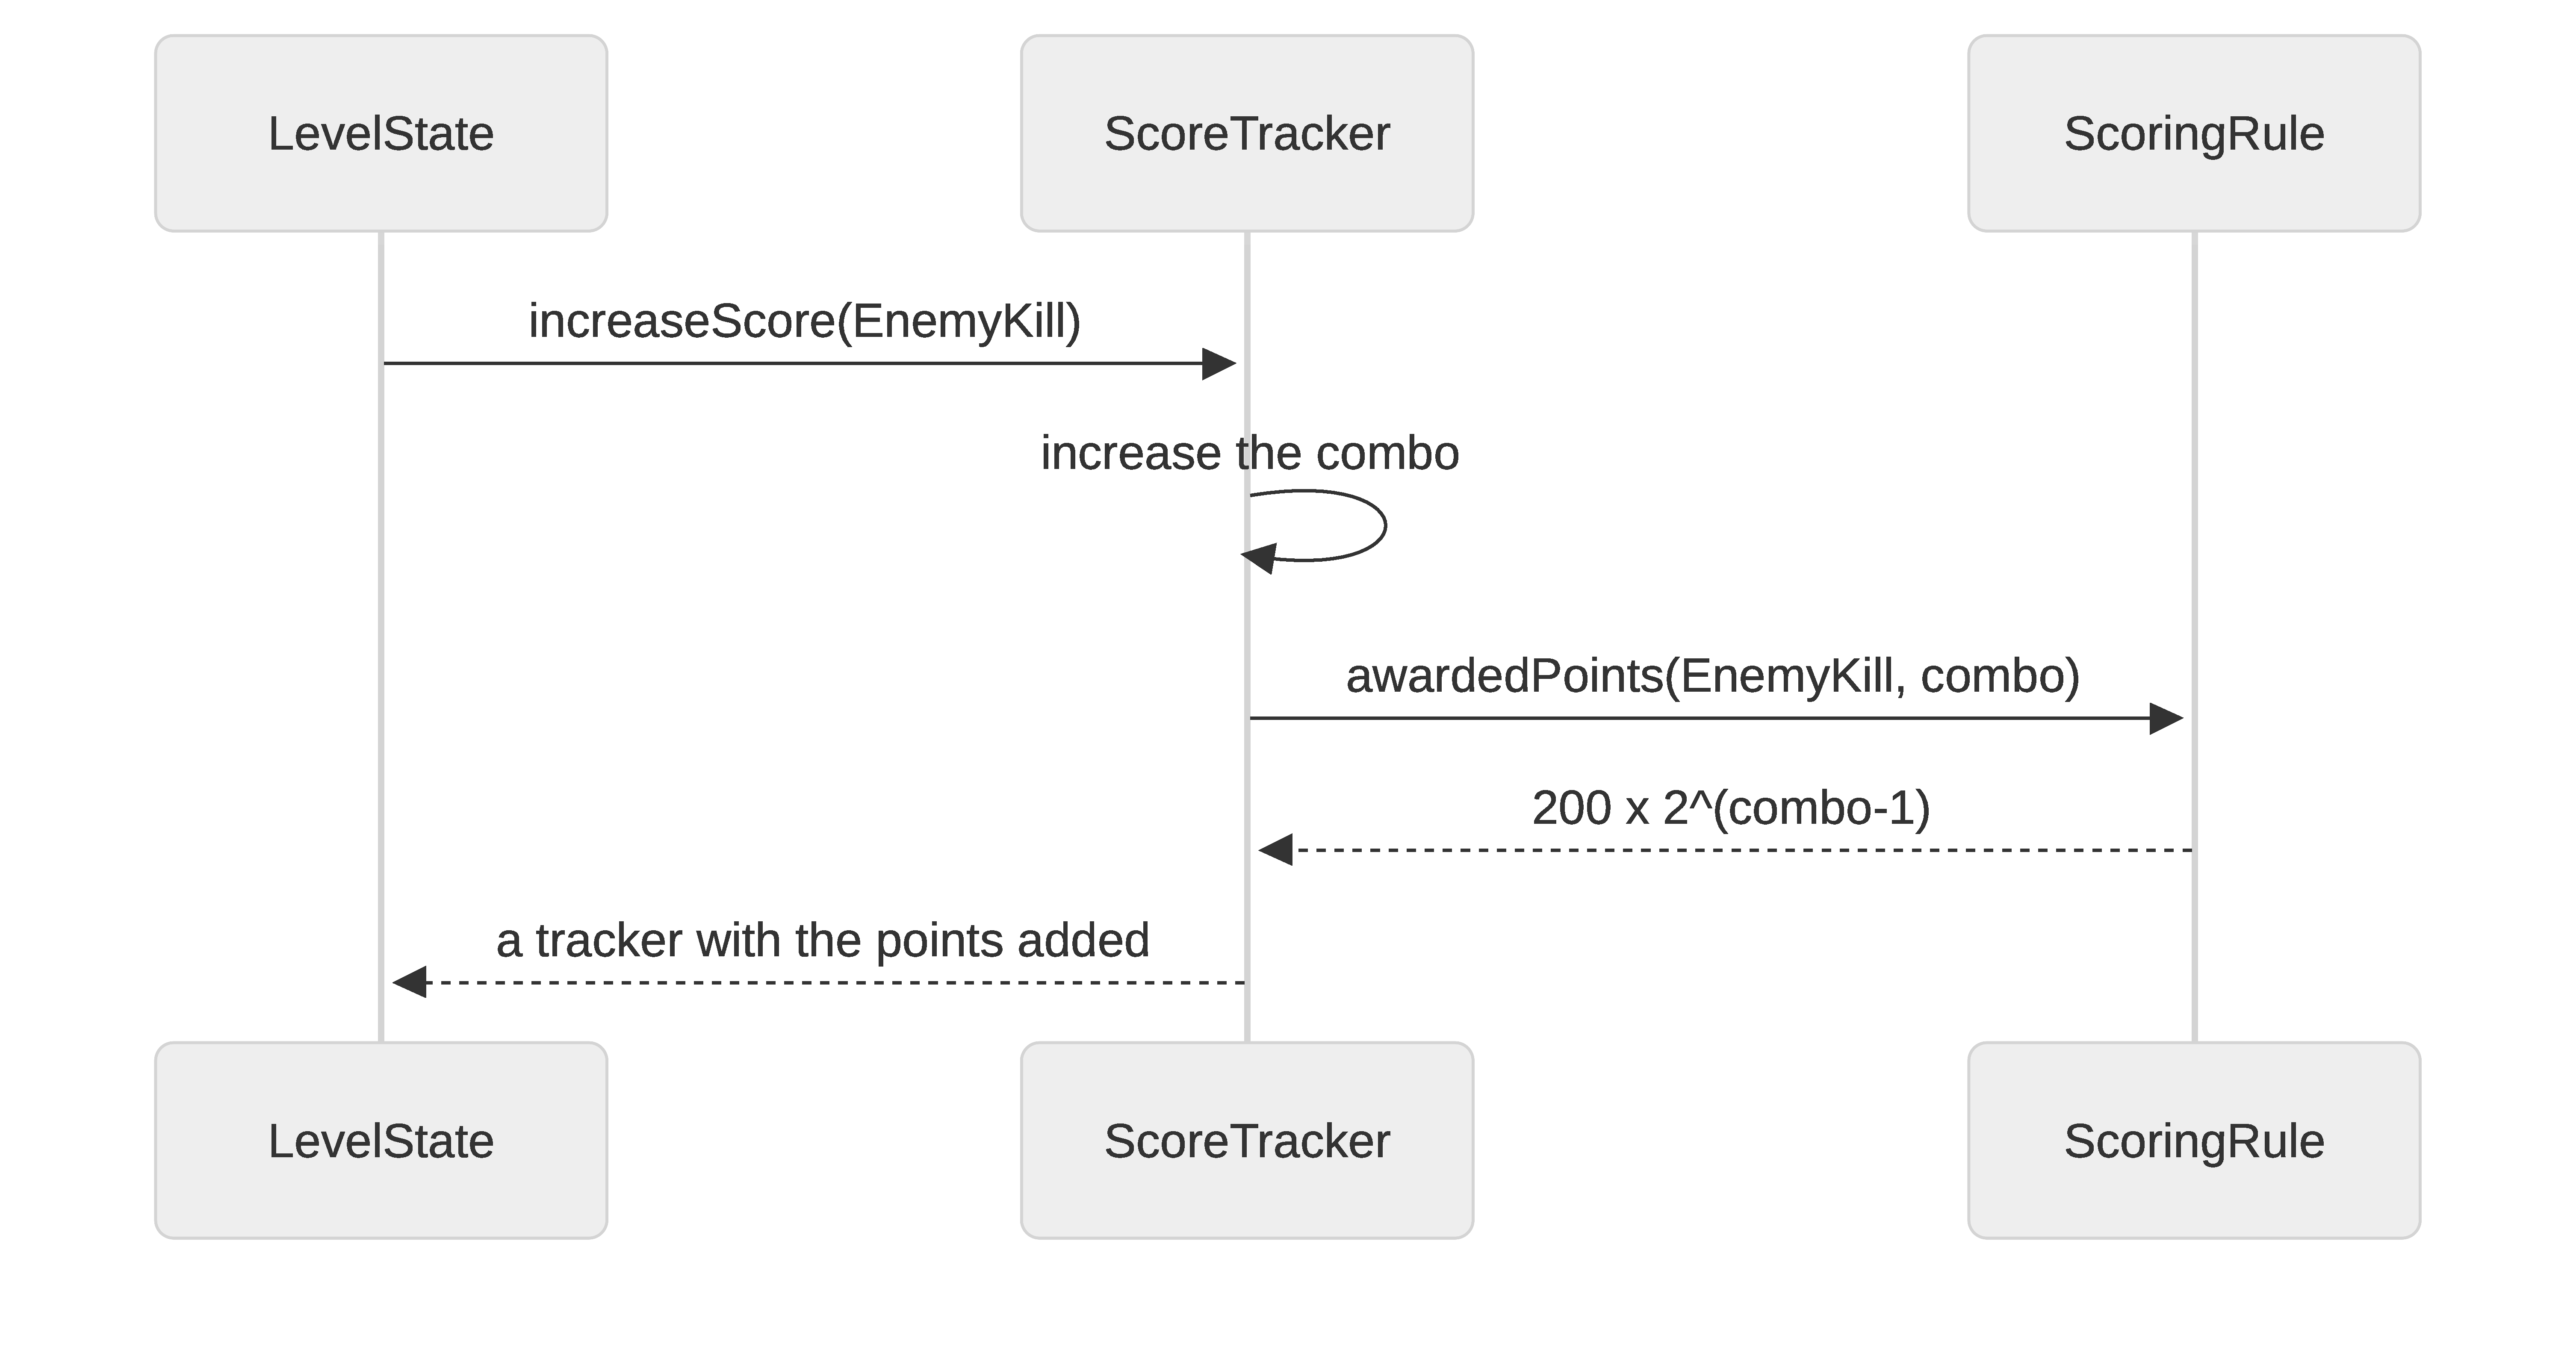
\includegraphics[width=0.9\textwidth]{../docs/uml/ComboIncreaseDiagram.pdf}
    \caption{The combo count is increased before the event is priced, so a kill counts towards its own multiplier}
\end{figure}

\section{Alex Santini}

My main implementation work focused on two boundaries that are essential to a reliable maze game: transforming a
textual maze into a \textbf{playable domain value}, and making enemies take \textbf{deterministic decisions} within
that maze. I also implemented the Timed and Survival modes, save/load support, and the CI checks used by the team;
the following sections concentrate on maps and AI because they contain the most substantial modelling and algorithmic
work.

\subsection{Maps as a validated input pipeline}

A map is authored as a UTF-8 ASCII file, but the game model must never depend on arbitrary text. I therefore split
map handling into three steps with different responsibilities:

\begin{enumerate}
  \item \texttt{MapLoader} is the only step that performs file I/O. It returns either the file text or a
  \texttt{MapLoadError}.
  \item \texttt{MapParser} is pure: it translates supported symbols into tiles and returns either a \texttt{RawMap}
  or a list of syntactic errors.
  \item \texttt{MapValidator} is pure: it checks gameplay invariants and returns either a \texttt{ValidatedMap} or
  a list of semantic errors.
\end{enumerate}

The resulting types make an invalid intermediate state visible at the boundary. \texttt{RawMap} is deliberately not
accepted by \texttt{LevelState}; only a \texttt{ValidatedMap}, containing the unique player spawn, enemy spawns,
collectibles, and paired teleports, can start a level. The application composes the pure stages with \texttt{Either},
turning domain errors into actionable messages only at the file-system boundary:

\begin{lstlisting}
private def read(text: String): Either[String, ValidatedMap] =
  for
    raw <- MapParser.parse(text).left.map(_.map(spelled).mkString("; "))
    maze <- MapValidator.validate(raw).left.map(_.map(spelled).mkString("; "))
  yield maze
\end{lstlisting}

This separation is useful both for robustness and for testing. A parser test never needs a file, a validation test can
construct a small \texttt{RawMap} directly, and an integration test can exercise the complete pipeline. It also keeps
the domain independent from paths, encodings, and \texttt{IOException}.

\subsection{Playability is a graph property}

Parsing checks whether text is well formed; it cannot determine whether a game can actually be completed. The
validator therefore inspects the rectangular grid once to collect its structural elements and checks that it has a
closed border, exactly one player spawn, at least one standard collectible, and at least one enemy. It pairs
teleports according to their documented codes and accumulates independent structural errors, so a map author can
correct several mistakes in a single attempt.

Once the structure is sound, \texttt{MapReachability} performs breadth-first search from the player spawn over
walkable orthogonal neighbours. A valid teleport pair contributes two directed graph edges, one in each direction.
The same traversal consequently proves that every required collectible and enemy can be reached even when the only
route crosses a teleport. This is stronger than checking local tile placement: an isolated but syntactically valid
collectible would otherwise make a level impossible to win.

\begin{center}
  \small
  \begin{tabular}{|p{2.3cm}|p{3.1cm}|p{3.2cm}|p{3.2cm}|}
    \hline
    \textbf{Stage} & \textbf{Input} & \textbf{Success} & \textbf{Failure} \\
    \hline
    \texttt{MapLoader} & \texttt{Path} & UTF-8 text & \texttt{MapLoadError} \\
    \hline
    \texttt{MapParser} & text & \texttt{RawMap} & \texttt{List[MapParseError]} \\
    \hline
    \texttt{MapValidator} & \texttt{RawMap} & \texttt{ValidatedMap} & \texttt{List[MapValidationError]} \\
    \hline
  \end{tabular}
\end{center}

The map suite was developed test-first. \texttt{MapParserSpec}, \texttt{MapLoaderSpec}, and
\texttt{MapValidationSpec} cover malformed rows, unsupported symbols, spawn cardinality, borders, teleport pairing,
and reachability; \texttt{MapPipelineSpec} verifies their composition. In particular, tests cover entities and
collectibles that are reachable only through a teleport, which protects the intended graph semantics rather than
only the ordinary grid case.

\subsection{Enemy AI as a deterministic strategy}

Enemy AI is part of the domain model, not of rendering or the game loop. I introduced
\texttt{EnemyMovementStrategy} as the narrow abstraction through which an enemy selects its next cell:

\begin{lstlisting}
trait EnemyMovementStrategy:
  def nextMove(context: EnemyMovementContext): Option[Position]
\end{lstlisting}

The context is an immutable value containing the enemy position, current and previous player positions, the
\texttt{ValidatedMap}, whether a teleport may be used, and an optional remembered target. A strategy returns
\texttt{None} when no movement is possible; it never mutates an enemy, reads global state, or accesses the UI. This
keeps each decision reproducible from its input and lets strategies be tested with a hand-built map.

\texttt{EnemyAiStage} owns orchestration. On each tick it leaves moving enemies unchanged, asks
\texttt{EnemyStrategySelector} for the strategy associated with an idle enemy kind, builds the context, retains any
strategy memory, and converts the selected next position into a legal entity movement. The stage is itself injected
into \texttt{LevelState.pipeline}, so tests may replace it without constructing a different game loop.

\begin{figure}
  \centering
  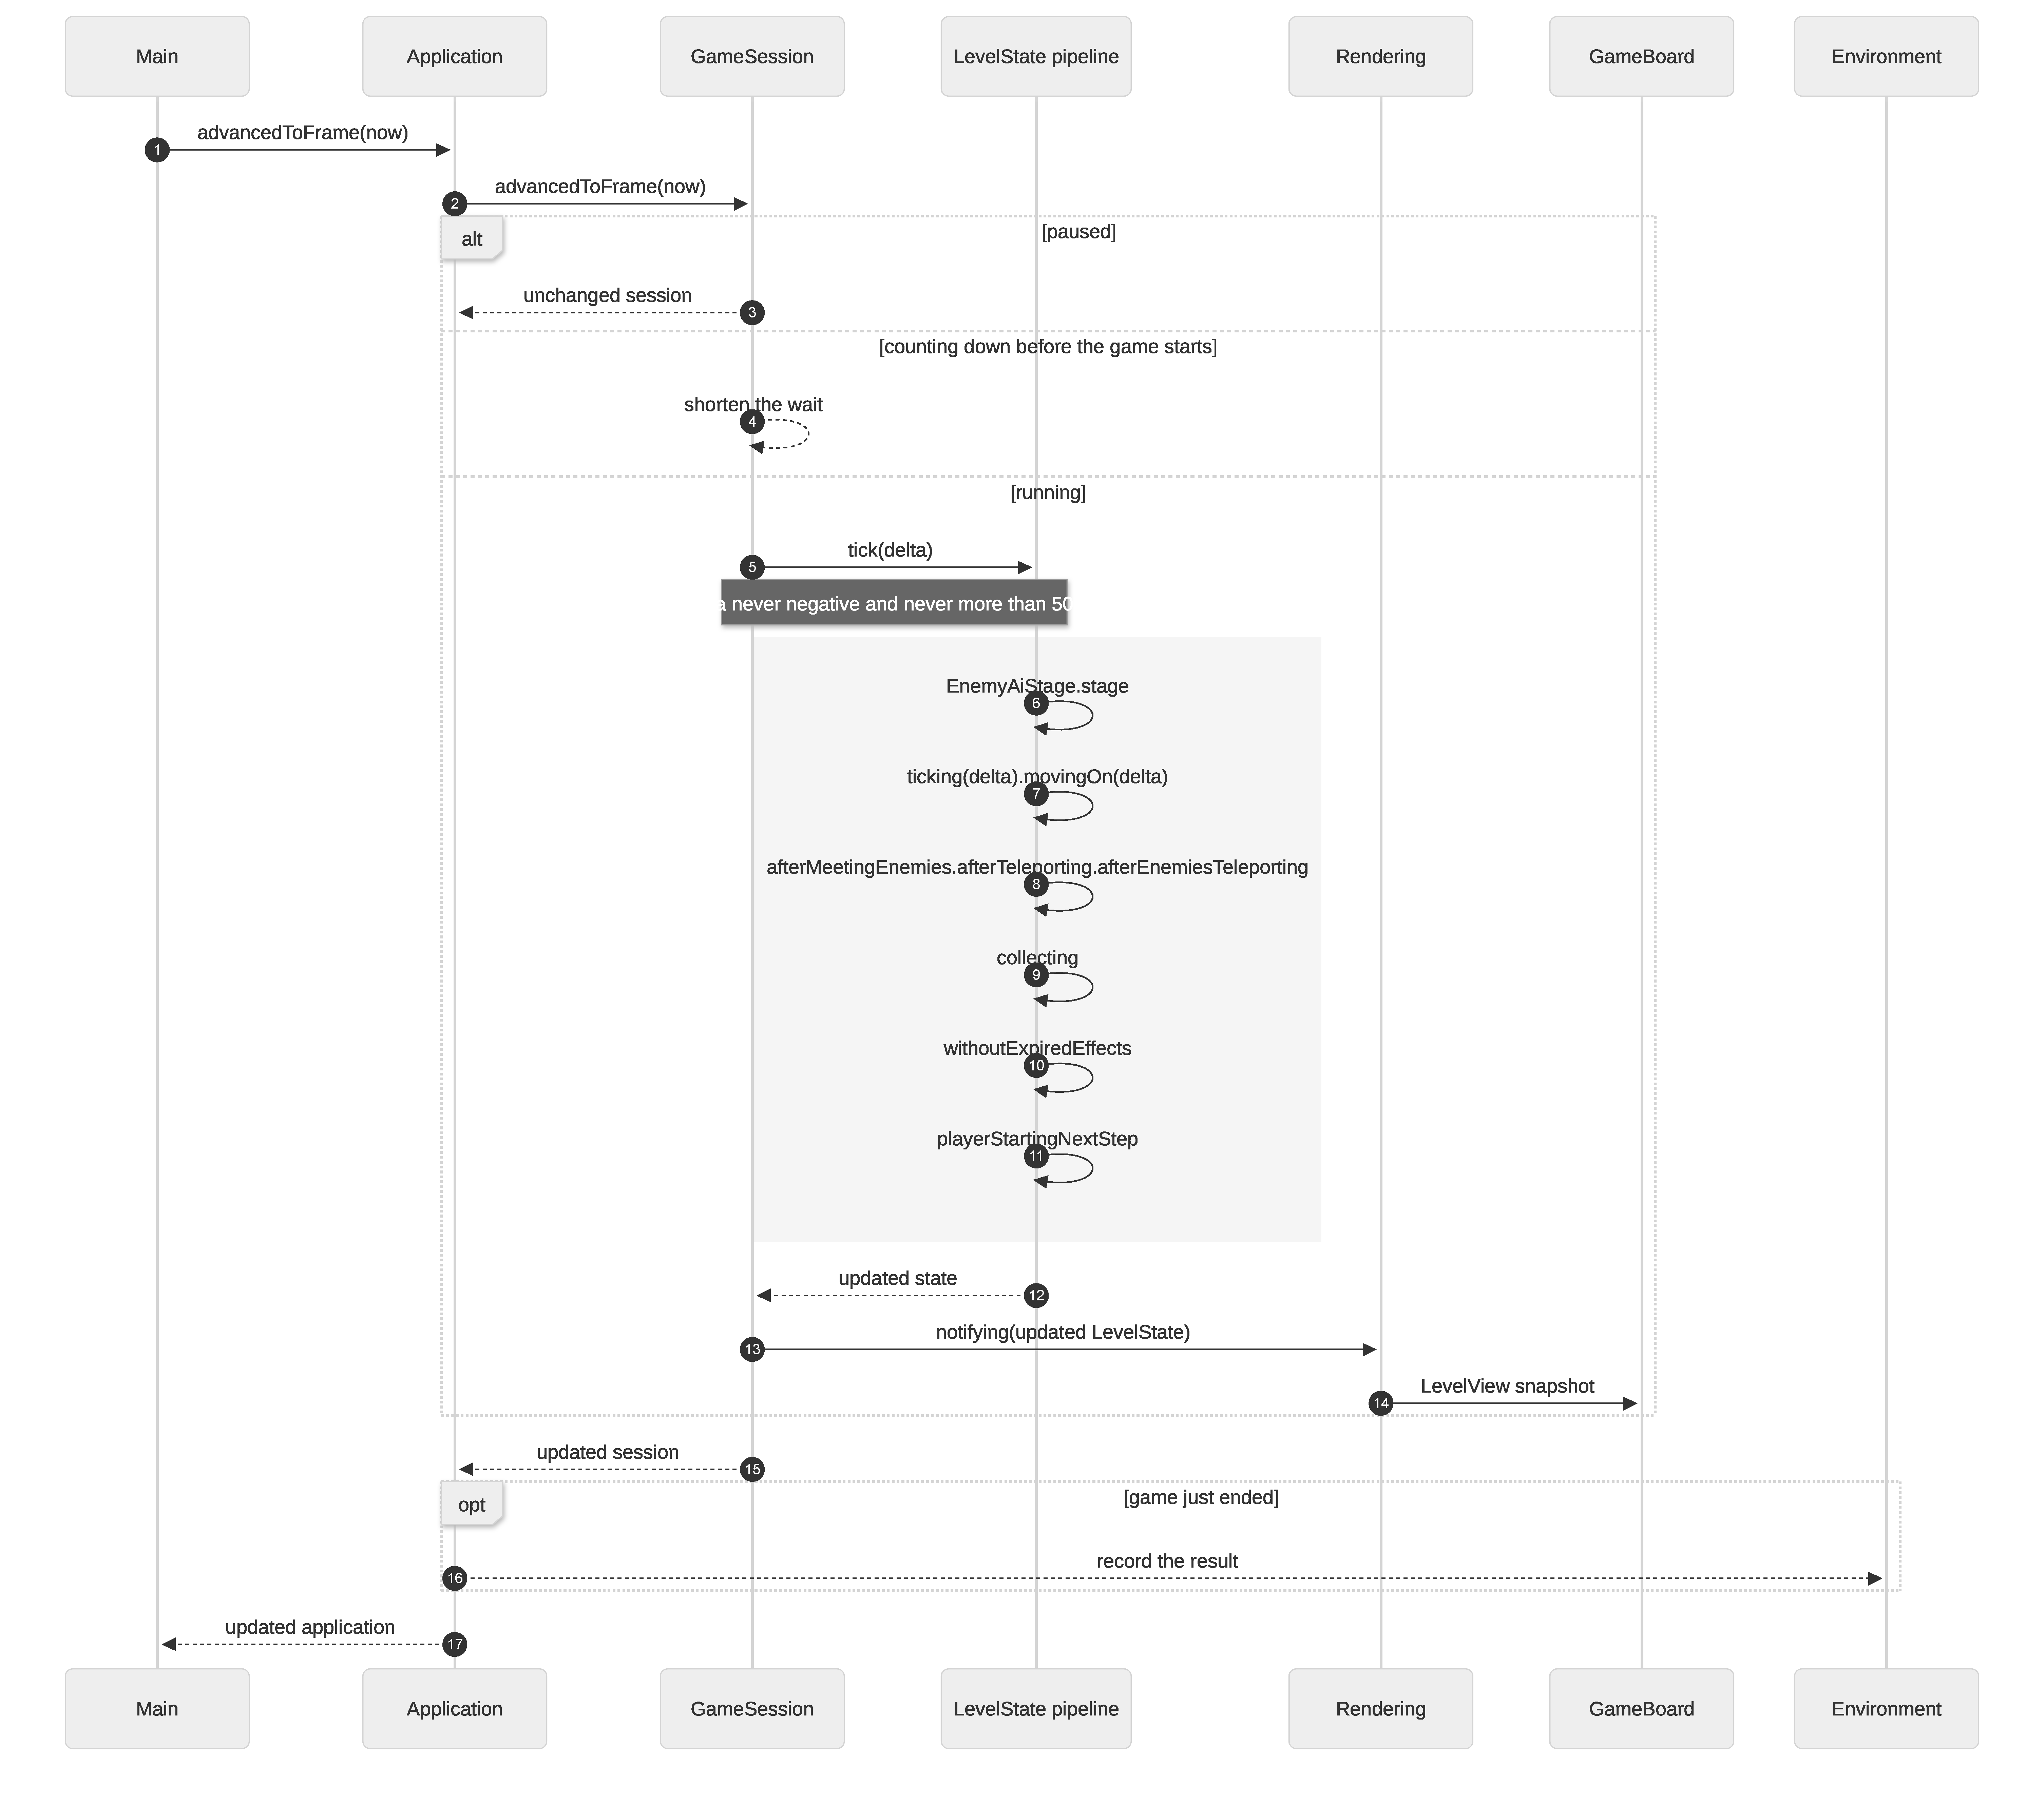
\includegraphics[width=0.92\textwidth]{../docs/uml/TickPipeline.pdf}
  \caption{The AI stage is the first domain stage of a tick. It proposes movement; later stages retain responsibility
  for movement progress, collisions, teleports, collection, effects, and the next player request.}
\end{figure}

\subsection{Path finding, anticipation, and teleport semantics}

The common \texttt{EnemyMovement} module contains the navigation policy shared by every strategy. It enumerates
walkable neighbours in a fixed order and uses a tail-recursive breadth-first search over immutable
\texttt{Queue}, \texttt{Vector}, and \texttt{Set} values. The first discovered path is therefore a shortest path,
and equal alternatives are resolved deterministically rather than by timing or randomness.

\texttt{DirectPursuitStrategy} takes the first step of that shortest path towards the player's current cell.
\texttt{PlayerAnticipationStrategy} derives a unit direction from the player's current and previous cells, projects
the player up to two walkable cells ahead, then chooses the legal move with the smallest shortest-path distance to
that prediction. If the player is stationary or the previous position is unavailable, it targets the current position;
if the projection meets a wall, it stops at the last walkable cell instead of predicting an invalid target.

Teleports are part of navigation rather than an exceptional afterthought. When allowed, the paired endpoint is added
to the candidate moves and can shorten a BFS route. After an enemy uses a teleport, its context disallows another
teleport at the origin until it has stepped away; this prevents an enemy from bouncing forever between paired cells.
The implementation and tests therefore share one semantics for ordinary movement, shortest paths, and teleports.

\subsection{Extension and verification}

The strategy boundary keeps an additional enemy behaviour local: implement \texttt{EnemyMovementStrategy}, reuse the
shared navigation primitives where appropriate, test the decision, and add a selector mapping only when the behaviour
is chosen from \texttt{EnemyKind}. The independently developed \texttt{PatrolStrategy} follows precisely this route,
which demonstrates that the original abstraction was sufficient without changing the update pipeline.

The AI tests cover valid moves, shortest paths, prediction, deterministic ties, teleport routing, the
no-immediate-return rule, selector mapping, and stage integration. Together with the map tests, they exercise the two properties
that matter most for these contributions: untrusted map data cannot enter play unchecked, and the same valid state
always produces the same enemy decision.

\subsection{Other contributions}

Outside these two main areas, I implemented \texttt{Timed} and \texttt{Survival} game modes, including the cap that
keeps Survival enemies no faster than the player's base speed. I implemented game saving and loading, where a saved
maze is reconstructed through the same parser and validator rather than trusted as persisted state. Finally, I set up
the project CI workflows for compilation, tests, scalafmt, report generation, and the delivery archive; this made the
repository continuously buildable and gave pull requests an objective integration gate.
